\documentclass[12pt]{article}

\usepackage[margin=1in]{geometry}
\usepackage{graphicx}
\usepackage{booktabs}
\usepackage{amsmath}
\usepackage{hyperref}
\usepackage{setspace}
\usepackage{caption}
\usepackage{natbib}
\usepackage{float}

\doublespacing
\graphicspath{{figures/}}

\title{Technical Report: Investigating Binge Drinking and Military Service}
\author{Connor Durand}
\date{}

\begin{document}

\maketitle

\begin{abstract}
It is a general stereotype that those who are serving or have served in the military are prone to alcohol related issues. Our research aims to build off current literature and establish an association between military service and binge drinking utilizing logistic regression. Current research has found a link with binge drinking and an individual's activity level for college age students but does not focus on the relationship with the military. When exploring the data, we find a potential interaction between military service and activity level. However, using a nested ANOVA difference in models' analysis we found no significant improvement in using the interaction term in our logistic regression. Our results demonstrated a lack of association between military service and binge drinking at the 0.05 significance level, but adequate association at the 0.1 level. Income and having an education level of high school or higher indicated stronger association and greater odds of being a binge drinker. However, our model suffered from extreme validity concerns, leading to potential inaccuracies. This research prompts further investigation into the association, with emphasis on improving the control variables to include more quantitative measures.
\end{abstract}

\newpage

\section{Introduction}

This research seeks to determine if there is an association between military service and binge drinking after accounting for income, physical activity level, and education level. Previous research has established that military service members have hazardous alcohol usage levels than civilians. Meadows et.\ al's research utilized logistic regression to analyze binge drinking in military service based off perceived alcohol culture while controlling for a magnitude of other factors. Some of the controlling factors warranted statistical significance in their model, such as education \citep{meadows2023culture}. Based on supplementary findings from their research, similar controls will be utilized. We will expand on their results by including additional controls, such as activity level, as explored by Dunn et.\ al.

Dunn used the 1995 National College Health Risk Behavior Survey to assess whether binge drinking, and other risk behaviors were influenced by college students' physical activity levels. They found that more active students being more prone to binge drinking \citep{dunn2003effects}. With a perception of high physical activity within military service, our research seeks to clarify whether military service, after controlling for miliary service (along with other factors) identifies a similar positive association with binge drinking. We plan to investigate this relationship using logistic regression. Through anecdotal experiences and societal stereotypes, it is hypothesized that military service will be positively associated with binge drinking.

\section{Data}

For this study, we will be using data from the August 2021--August 2023 National Health and Nutrition Examination Survey (NHANES). Data from the Demographic and Questionnaire sections of the survey were compiled and merged through a unique respondent sequence number. The sample design consists of multi-year, stratified, clustered four stage samples. The sample represents noninstitutionalized civilian population within the 50 states (to include the District of Columbia), with respondents aging from 0 to 80+ years old \citep{nhanes2023}. However, with our variables in consideration, we limited the observational units to adults between the ages of 21 and 80 in the United States for a final sample size of ($n=1477$).

The response variable is whether or not an individual is considered a binge drinker, self-identified on the survey as drinking more than 4/5 drinks in a 2-hour period 3--6 times or more in the past year. Our response variable, binge drinker, was classified as binary, with either yes (1) or no (0) responses. The main explanatory variable in question is whether or not the individual has served active duty in the U.S.\ Armed Forces, self-identified as ever serving on activity duty in the U.S.\ Armed Forces, military Reserves, or National Guard. Similarly, our researched explanatory variable, military service, is binary with yes (1) and no (0) response.

The potential confounding variables of income, physical activity level, and education level had to be adjusted from their raw survey outputs for use in our model or are less intuitive than the variable title suggest. The control used for income is a ratio of the induvial survey family income to the poverty level. This ratio ranges from 0 to 4.99, with the survey capping responses greater than 5 to the value of 5. An individual's physical fitness level was assessed through their response to a series of two questions, one asking for frequency of moderation leisure time physical activities, and the other asking for unit of measurement (example response, Q1: 3 times, Q2: per month). These responses were then compiled and converted into a number of times per week, not considering the duration of a physical activity. Due to the complexity of the two-part questions, some responses were extreme and unfeasible, while others may have been underreported. To combat this, after removing unfeasible outputs, individuals were categorized into a medium, low, or high physical activity level group, classifying it a categorical variable. Education level did not suffer from issues of extreme and unfeasible values, however, to ensure each group had enough samples, we split the sample into two district groups of individuals with less than high school education, and those with greater than high school education, creating a binary control variable. See Table~1 in Appendix~A.

\section{Methods}

After we cleansed our data, we explored our explanatory and control variables by grouping them as either a binge drinker or not binge drinker, see Table~2 in Appendix~A. We identified that income was significantly different between binge and non-binge drinking groups at the 5\% significance level, indicating its importance as a control in the regression.

We then sought to identify any potential interactions between our variables of interest. Using intuition and prior knowledge of the military profession, we tested the interaction between physical activity level and binge drinking through an interaction plot, see Figure~3 in Appendix~B. Our interaction plot depicted nonparallel slopes between those with military service and those without military service, with changing physical activity levels on proportion of binge drinkers. Due to this relationship, we recognized that interaction between the two variables may exist and should be explored in a model. We also attempted to the interaction between income and military service utilizing an interaction plot, however, revealing parallel slopes indicated no suggestion of an interaction.

Based off of the data exploration, we created two logistic models to provide interpretability of a binary dependent variable. In order to utilize logistic regression, the following validity conditions were tested through the creation of a Normal Q-Q Plot, Histogram of Residuals plot, and Residuals vs Predicted values plot. Prior to testing, we assumed that there is no curvature in the residuals vs.\ predicted values graph (linearity), observations are independent of each other (independence), the residuals are approximately normal, and there is approximately equal variance in the residuals.

The first model is the general form:
\begin{equation}
\text{logit}(\pi_i) = \beta_0 + \beta_1 \cdot \text{Military}_i + \beta_2 \cdot \text{Income}_i + \beta_3 \cdot \text{ActivityLevel}_i + \beta_4 \cdot \text{Education}_i
\end{equation}

We also created an interaction model with an added military and activity interaction term:
\begin{equation}
\text{logit}(\pi_i) = \beta_0 + \beta_1 \cdot \text{Military}_i + \beta_2 \cdot \text{Income}_i + \beta_3 \cdot \text{ActivityLevel}_i + \beta_4 \cdot \text{Education}_i + \beta_5 \cdot (\text{Military}_i \times \text{ActivityLevel}_i)
\end{equation}

In this model, $\text{logit}(\pi_i)$ represents the log odds of an individual being a binge drinker. The baseline of our model, demonstrated by $\beta_0$, is the log-odds of being a binge drinker for an individual with no military service, zero income, high physical activity, and less than a high school education. $\beta_1$ is the increase in log-odds associated with having served in the military. $\beta_2$ represents the increase in log-odds for each one-unit increase in income. $\beta_3$ represents the change in log-odds for each decrease in physical activity level from high physical activity level. $\beta_4$ represents the increase in log-odds associated with having greater than high school education compared to less than high school education. $\beta_5$, which only appears in the interaction model, represents the increase in log-odds for an interaction between physical activity level and military service.

After compiling our two logistical regression models, we compare them and determine which model is best, using a nested ANOVA difference in models' chi squared test. With the identified `best' fitting model, we then computed the predicted probabilities of outcome status for each observation in the dataset. We then selected a cut-off value of 0.35 to classify whether predicted probabilities were failures and successes and determine the classification rate of our model. We opted for this cut-off value since Table~2 identified unequal groups of binge (1) and not binge drinkers (0), with a mean value of .308, in an attempt to get a roughly equal number of individuals classified as binge and non-binge drinkers.

\section{Results}

After regressing our general and interaction logistical regression models, we found the fitted models. The fitted general model was:
\begin{equation}
\text{logit}(\hat{\pi}) = -1.267 + 0.639 \cdot \text{Military} - 0.163 \cdot \text{Income} + 0.134 \cdot \text{ActivityMed} - 0.045 \cdot \text{ActivityLow} + 0.540 \cdot \text{AboveHS}
\end{equation}

And the fitted interaction was:
\begin{multline}
\text{logit}(\hat{\pi}) = -1.218 + 0.288 \cdot \text{Military} - 0.162 \cdot \text{Income} + 0.016 \cdot \text{ActivityMed} - 0.134 \cdot \text{ActivityLow} \\
+ 0.539 \cdot \text{AboveHS} + 0.595 \cdot \text{Military:ActivityMed} + 0.378 \cdot \text{Military:ActivityLow}
\end{multline}

We then compared the results using an ANOVA comparison of Deviance resulting in a Chi squared p-value of 0.2938, indicating that we do not have significant evidence to suggest that the interaction model was significantly better than the general model. Because of this, we decided to focus our attention on the general model.

To check our validity conditions of the general model, we examined the Normal Q-Q, Histogram of Residuals, and Residuals vs Predicted values plots. As shown in Appendix~C, our model does not meet validity conditions. The Normal Q-Q Plot in Figure~2 still shows curvature, failing the linearity constantly. Additionally, Figure~3, the Histogram of Residuals depicts the residuals as skewed right, failing the normality constraint. With this considered, the results from our regression should be carefully evaluated, as it may report inaccuracies.

Additionally, we computed the Odds Ratio and 95\% confidence interval for our coefficients, See Table~3 in Appendix~B. The results revealed that the odds of being a binge drinker for those who served in the military are 0.639 times the odds of those who have never served in the military. This estimate was significant at the 0.1 significance level. The coefficients of income and above high school education were both significant at the 0.001 significance level. The coefficients reveal that the odds of being a binge drinker decrease by 0.850 times for each 1 unit increase in education, and having above a high school level of education decreases the odds of being a binge drinker by 0.583 times those who have less than a high school level of education.

However, the classification rate of our model was worse than expected. Our model had an accuracy rate of 65.81\%. However, always predicting an individual as a non-binge drinker warrants a accuracy rate of 69.19\%. Comparing our model to always predicting the individual as a non-binge drinker resulted in a p-value of 0.9976, indicating the generalized model did not perform significantly better. See Figure~5 and 6 for the Predicted Probability vs Actual Status with 0.35 as Cutoff and Confusion Matrix R Output respectively. Table~5 and Figure~6 also indicate that our model predicts those who are non-binge drinkers with more accuracy than those non binge drinkers.

\section{Discussion}

The results indicated a potential association in the opposite direction as originally hypothesized, revealing that military service may be negatively associated with binge drinking. While our explanatory variable of interest did not achieve statistical significance at the 0.05 significance level, our model is still able to provide insight into the relationship and expand the academic discussion of binge drinking on military service. While we fail to support that there is an association between military service and binge drinking after accounting for income, physical activity level, and education level, (at the 0.05 significance level), the closeness to significance provides hope for future studies.

The data used provides excellent generalizability through the random sampling measures across the US but appears to have hindered the strength of evidence. Limitations with data severely impacted our ability to obtain purely quantitative counts of physical activity level. Additionally, the general model used failed to pass necessary validity conditions, weakening the interpretability and accuracy of the results. The model failed to outperform an algorithm that classified all sampled individuals as non-binge drinkers with a 0.35 cut-off, limiting its applicability for classifying individuals both inside and outside the sampled population.

Future studies should attempt to use another metric of physical activity, that is not subject to being transformed into a categorical variable. Our research used the most recent NHANES survey (2021--2023) with limited collection due to COVID-19, utilizing a larger period of time may assist in providing numbers to previously low sample count groups, specifically those with military service. Due to the sourcing of the data, no ethical considerations are warranted by the use of the model. This research suggests that there may be an association between binge drinking and military service, but finer tuned control variables should be sought and used. If future research is able to confirm the negative association we identified, an analysis of the military's alcohol policy and attitudes may be applied to populations with higher binge drinking rates.

\section*{Works Cited}

\bibliographystyle{apalike}
\bibliography{references}

\newpage
\appendix

\section{Appendix A}

\begin{figure}[H]
\centering
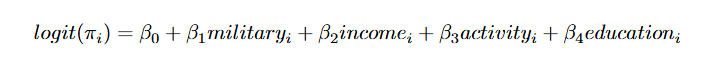
\includegraphics[width=\textwidth]{image1.png}
\caption{Table 1: Study Variables and Descriptions}
\end{figure}

\begin{figure}[H]
\centering
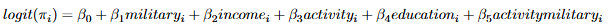
\includegraphics[width=\textwidth]{image2.png}
\caption{Table 2: Summary of Subject Characteristics by Binge Drinking Status}
\end{figure}

\begin{figure}[H]
\centering
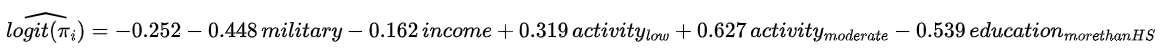
\includegraphics[width=\textwidth]{image3.png}
\caption{Table 2 (continued)}
\end{figure}

\section{Appendix B}

\begin{figure}[H]
\centering
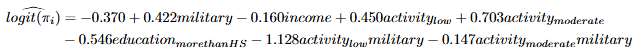
\includegraphics[width=\textwidth]{image4.png}
\caption{Figure 1: Interaction Plot -- Military Service and Physical Activity Level on Proportion of Binge Drinkers}
\end{figure}

\begin{figure}[H]
\centering
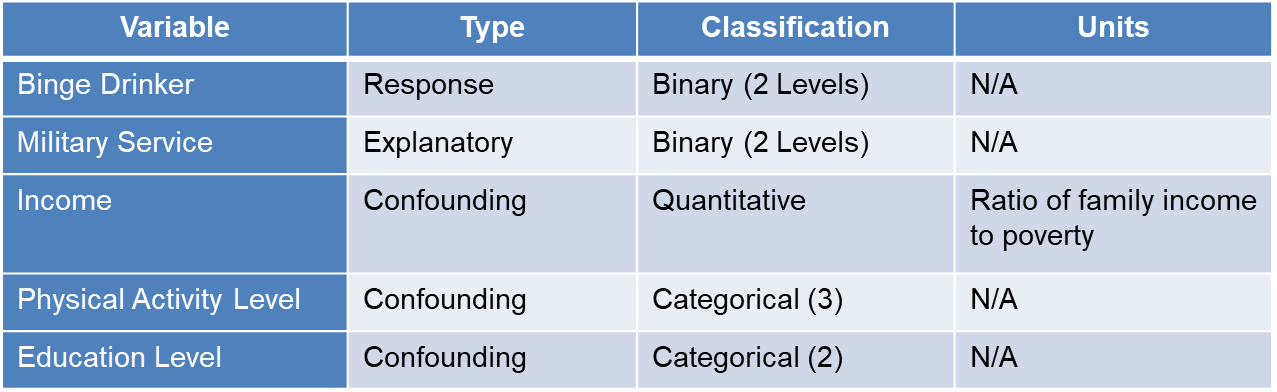
\includegraphics[width=\textwidth]{image5.png}
\caption{Table 3: Odds Ratios and 95\% Confidence Intervals for General Model Coefficients}
\end{figure}

\begin{figure}[H]
\centering
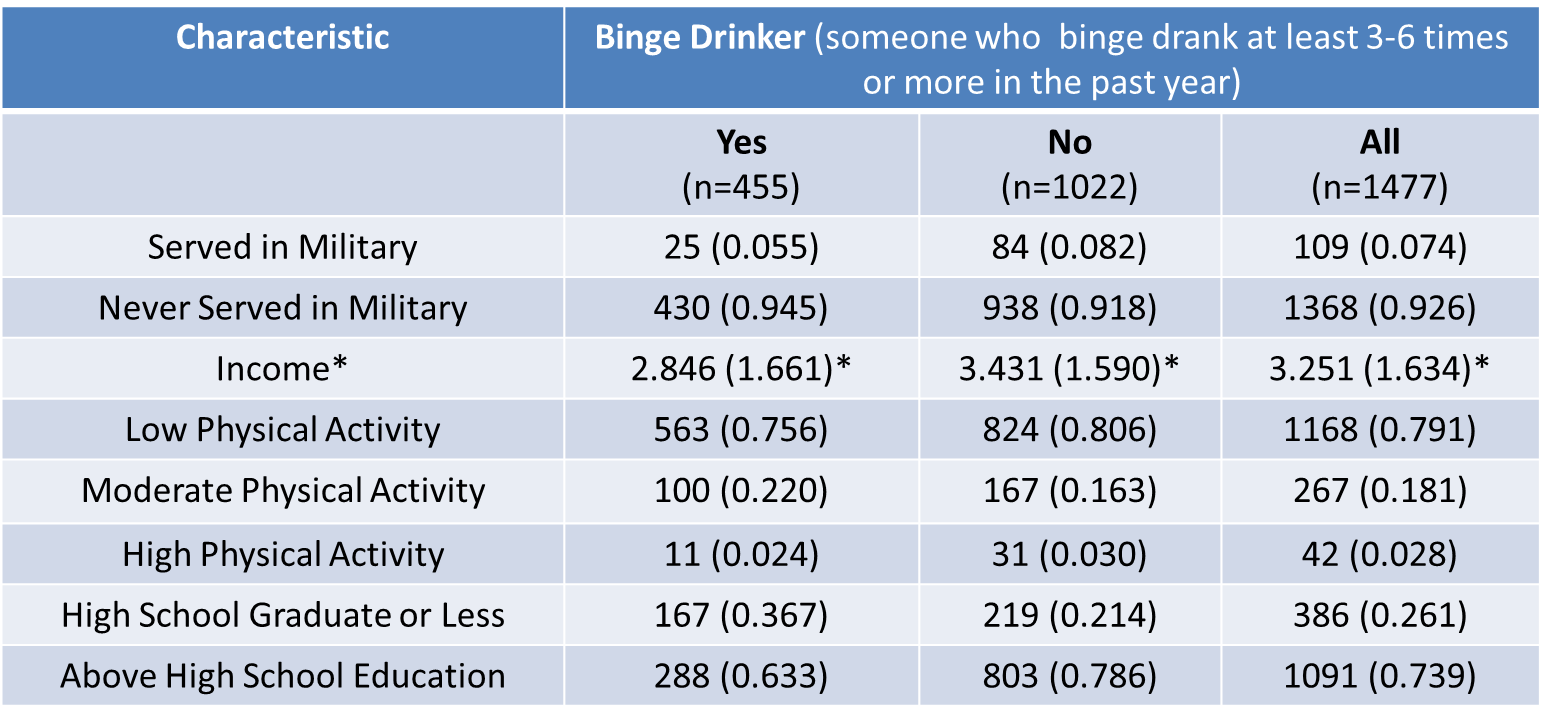
\includegraphics[width=\textwidth]{image6.png}
\caption{General Model Regression Output}
\end{figure}

\begin{figure}[H]
\centering
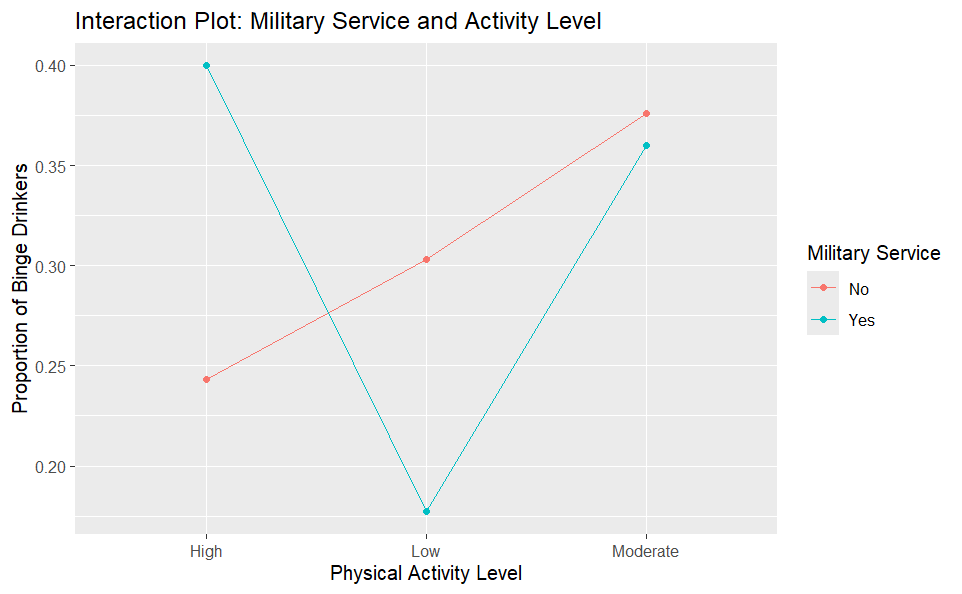
\includegraphics[width=\textwidth]{image7.png}
\caption{Interaction Model Regression Output}
\end{figure}

\begin{figure}[H]
\centering
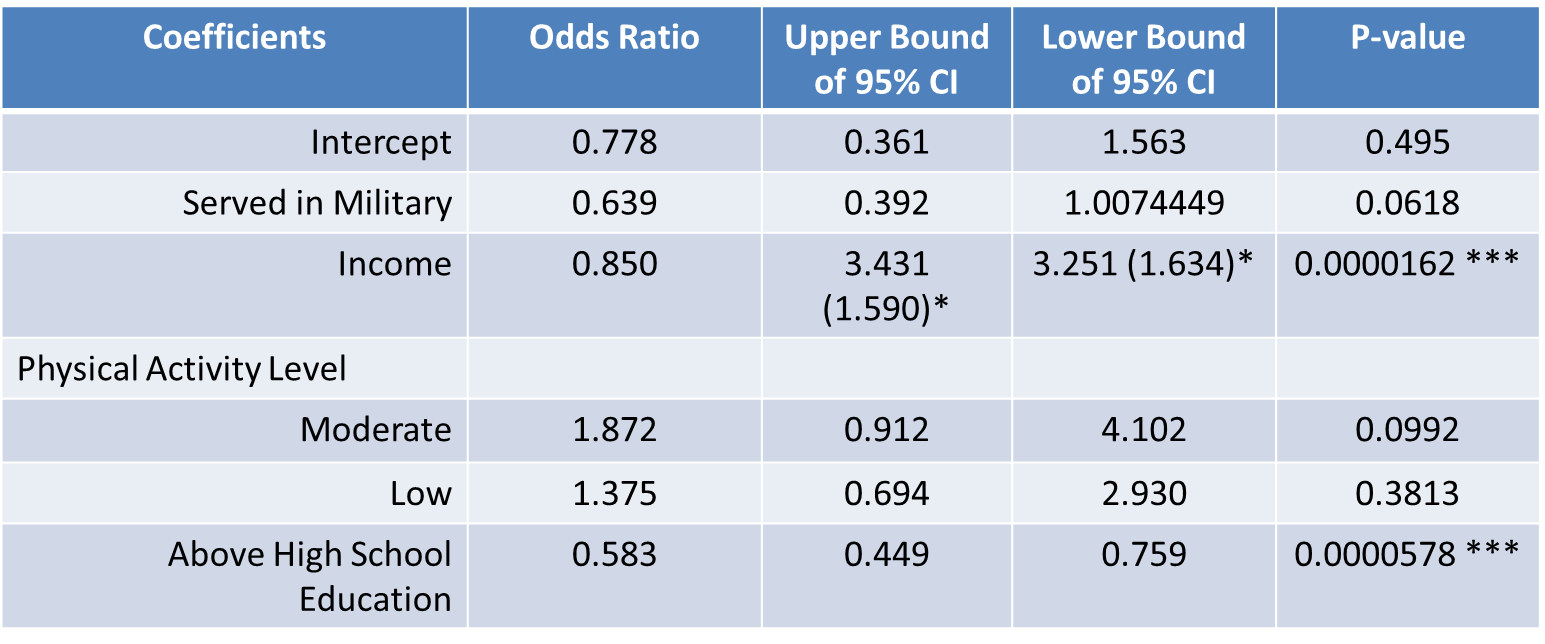
\includegraphics[width=\textwidth]{image8.png}
\caption{ANOVA Comparison of Deviance Output}
\end{figure}

\section{Appendix C}

\begin{figure}[H]
\centering
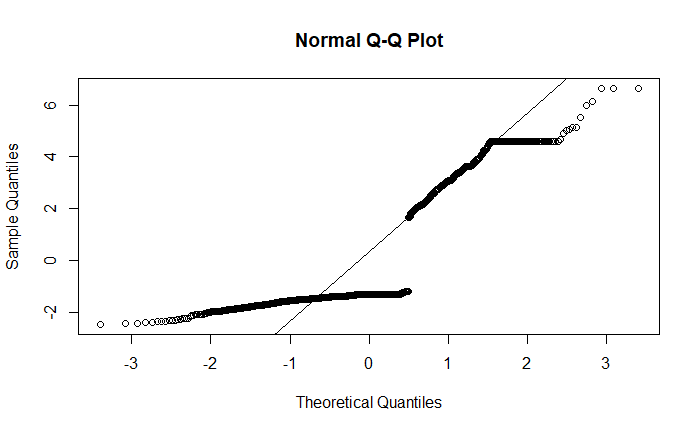
\includegraphics[width=\textwidth]{image9.png}
\caption{Figure 2: Normal Q-Q Plot of Residuals}
\end{figure}

\begin{figure}[H]
\centering
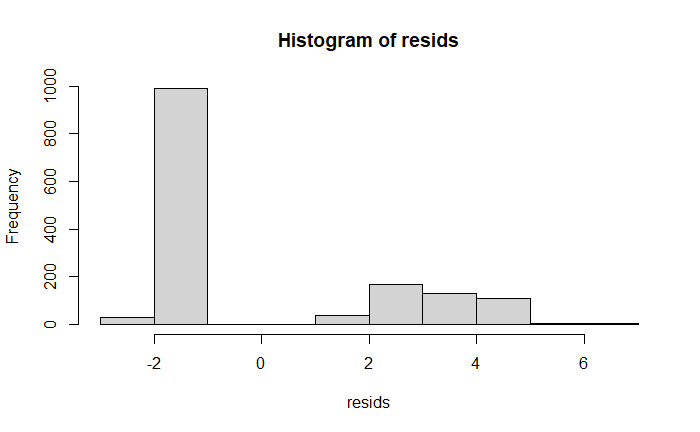
\includegraphics[width=\textwidth]{image10.png}
\caption{Figure 3: Histogram of Residuals}
\end{figure}

\begin{figure}[H]
\centering
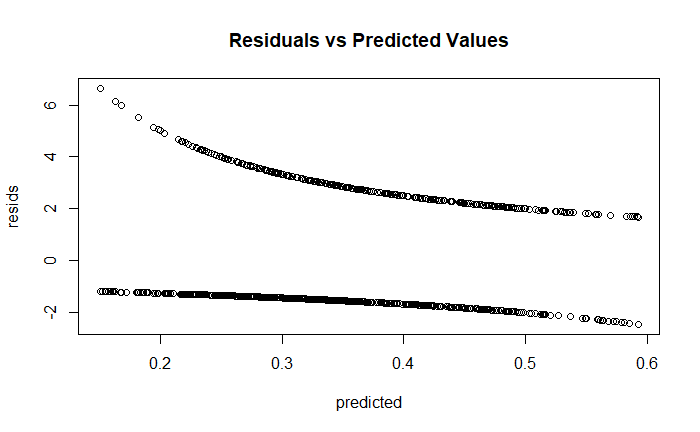
\includegraphics[width=\textwidth]{image11.png}
\caption{Figure 4: Residuals vs Predicted Values}
\end{figure}

\section{Appendix D}

\begin{figure}[H]
\centering
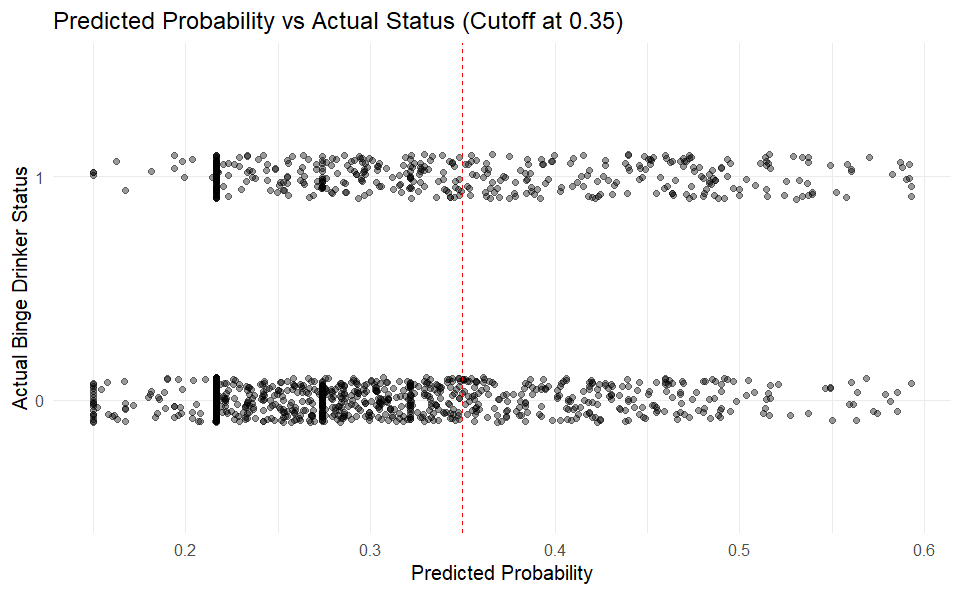
\includegraphics[width=\textwidth]{image12.png}
\caption{Figure 5: Predicted Probability vs Actual Status with 0.35 Cutoff}
\end{figure}

\begin{figure}[H]
\centering
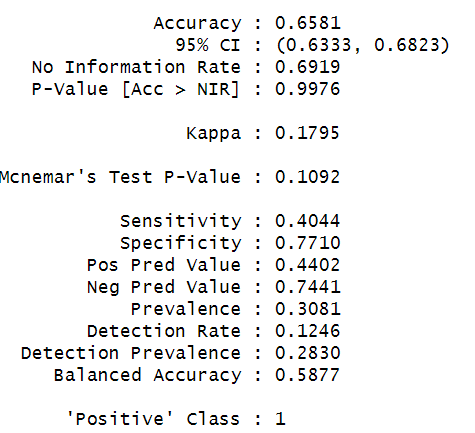
\includegraphics[width=\textwidth]{image13.png}
\caption{Figure 6: Confusion Matrix R Output}
\end{figure}

\begin{figure}[H]
\centering
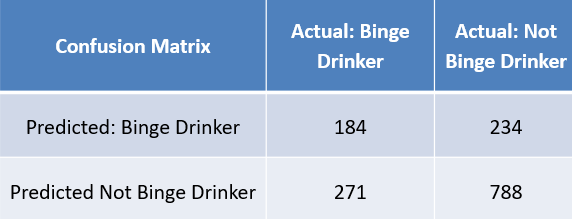
\includegraphics[width=\textwidth]{image14.png}
\caption{Table 4: Confusion Matrix Summary}
\end{figure}

\end{document}
